% UTF-8

% single-chapter commands
\documentclass{../thesis} \setcounter{chapter}{1} \begin{document}


\chapter{Analyse der Ausgangslage}

\section{OpenStreetMap: Alles für Alle}
Topographische Vermessungen führten ursprünglich nur zu relativ ungenauen Ergebnissen \cf[43]{Koh04}. Für die im 18.~und 19.~Jahrhundert erstmals durchgeführte systematische Landesaufnahme standen nur am Boden operierte Messinstrumente zur Verfügung. Bis in die zweite Hälfte des 20. Jahrhunderts waren der manuell horizontierte und abgelesene Theodolit und das Bandmaß die dabei primär eingesetzten Instrumente \cf[3–6]{WG06}. Deren Natur entsprechend ging dies mit einem immensen Aufwand an Arbeitskräften einher.

Die schiere Menge der eingesetzten Vermesser machte im Laufe der Zeit auch mit einfachen Instrumenten zufriedenstellende Ergebnisse möglich. In den letzten Jahrzehnten haben Photogrammetrie, Fernerkundung und satellitengestützte Ortsbestimmung das Vermessungswesen revolutioniert. Genauere Resultate ließen sich in kürzerer Zeit und so auch mit geringeren Kosten erreichen. \noref

% Ist die Kostendiskussion wirklich von Interesse? Eigentlich geht's ja nur um die ursprüngliche Motivation für OSM

Obgleich die Kosten geringer als zuvor sind, liegen sie nach wie vor in mehrstelliger Millionenhöhe allein für die amtlichen Geobasisdaten eines deutschen Bundeslandes \cf[3]{lgm05}.
% [lgm05 3 (LG München, Beschl. vom 9. Nov. 2005, Az. 21 O 7402/02, 3; in: GRUR 2006, 225)]
In Europa \noref herrscht heutzutage \cf[119]{Fis01} die Auffassung vor, dass diese solcherart mit Steuergeldern erhobenen Daten der Allgemeinheit nicht kostfrei zur Weiternutzung zur Verfügung gestellt werden, sondern die \emph{konkreten} Nutzenden zusätzlich Lizenzgebühren zahlen sollen \noref. Diese Lizenzkosten schränken den Nutzen amtlicher Geodaten nicht nur für kommerzielle Zwecke \cf[336]{Böh07}, sondern auch für Privatleute \noref erheblich ein \noref.

% [Egg99 \noref]

Heute haben selbst billige GPS-Empfänger eine Genauigkeit, welche die mancher Vermessung des 19. Jahrhunderts übertreffen kann \cf[346][\?]{WG06}. Die „freie Weltkarte“ \eyecatcher{OpenStreetMap} (OSM) \cf[3]{RT09} macht sich dies zu Nutze, um mit Hilfe zehntausender Freiwilliger eine weltweite Datenbank mit Geobasisdaten aufzubauen und nachzuführen (Volunteered Geographic Information, VGI) \cf[147, 154]{NZ12}. Im Gegensatz zu vielen amtlichen Geobasisdaten dürfen OpenStreetMap-Daten lizenzkostenfrei verwendet werden, auch für kommerzielle Zwecke \cf[217, 221\f]{RT09}.

% ODBL? -> 3rd ed

% fühlt sich alles _viel_ zu lang an … was davon brauche ich wirklich als Überleitung zu Fragmentierung und Process?
% straff kürzen, unbekannte Begriffe a la KV-Pair einfach in Fußnote packen…
% Oder wild ausdehnen, z. B. Verweis auf NoSQL-Prinzip hinsichtlich Flexibilität? … Nein, das ist nicht Aufagbe dieser Arbeit. Lieber noch mehr Verweise suchen.

Der Name OpenStreetMap mag fehlleitend sein, denn es handelt sich dabei nicht um eine Straßenkarte, sondern vielmehr um eine Geodatenbank mit Inhalten nahezu beliebiger Themen. Bei der Gründung von OSM im Jahr 2004 wurde auf das Festlegen starrer Klassifizierungsschemata oder Kartierschlüssel verzichtet. Statt dessen kann jedes Element in der Datenbank mit einer beliebigen Anzahl Attribute – sogenannter \term{tags} – versehen werden, die jeweils aus einem Schlüssel und einem Wert bestehen \term{(key-value-pair)}. \cf[56]{RT09}

% ways / relationen / fragmentierung !!

Syntax und Semantik der einzelnen \term{tags} werden bei OpenStreetMap seit der Gründung fortlaufend von den Beitragenden diskutiert, gestützt auf bisherige Erfahrungen. Die Diskussion findet vornehmlich im Internet statt; Ergebnisse werden öffentlich dokumentiert und in Software wie z.~B. Renderern implementiert. Wer neue Inhalte erfasst, orientiert sich oft an den bisher in der Datenbank üblichen oder im Web dokumentierten Konventionen. \cf[48]{Top09} \cf[17\f, 59–66]{RT09}

Gegenüber einer vor der Erfassung vereinbarten gemeinsamen Ontologie \cf[14]{GOS09} hat dieses System zur Folge, dass die zu OSM Beitragenden genau das erfassen, was sie persönlich interessiert und für wichtig halten. Jeder der Beitragenden entscheidet die Kriterien für die Erfassungsgeneralisierung für sich selbst. %Dies führt zu großen regionalen Unterschieden in Datendichte, -aktualität und -qualität.
% Regionalität ist nicht entscheidend für uns.

% Verweis auf Sch09 deckt schon vieles ab; Kne09 eher knapp, Beh11 noch knapper, Kla11 umständlich

Oft verfügen die OpenStreetMap-Daten über sehr hohen Detailreichtum. So könnten zum Beispiel für Teilstücke einer Straße \term{tags} für Tempolimits, Überholverbote, Fahrspurenanzahl, Oberflächenmaterial sowie -Qualität, Baujahr und mehr eingetragen worden sein. Veränderungen an diesen Attributen im Verlauf der Straße führen im OSM-Datenmodell zwangsläufig zu einer Fragmentierung in mehrere aufeinander folgende Linienabschnitte \term{(ways)}, jeweils mit unterschiedlichen \term{tags} \cf[57]{RT09}.

% "Detailreichtum entsprechend einer Grundkarte" (?) -> verdeutlicht, dass OSM ungeneralisiert ist

Baulich getrennte Fahrbahnen wie etwa Autobahnen bildet OpenStreetMap mittels zweier paralleler Einbahn-Linienzüge ab \cf[62]{RT09}. Dies ist eine in der Geoinformatik gängige Vorgehensweise \cf[2][\?]{Tho05}.

Sowohl die Fragmentierung als auch die parallelen Linienzüge führen zu Schwierigkeiten in der Weiterverarbeitung und Visualisierung \noref[Mig12 u. a.].
% Abbildungen:
% - Marker-Wucherung
% - stark unregelmäßige Plazierung von Namen \cf{Mig12}
% - Blitzer/Freistellung
% - Doppelnamen \cf{Mig12}
% o. ä.
Offensichtlich ist, dass eine Verkettung der Fragmente bzw. parallelen Linienzüge als Bestandteil des Datenmodells die Probleme wesentlich verkleinern, wenn nicht gar gänzlich lösen würde. Für eine hierarchisch orientierte Organisation wie etwa Vermessungsämter wäre eine solche Lösung naheliegend. Über \term{relations} ist dies auch in OpenStreetMap möglich \cf[57]{RT09}. Das oben beschriebene Fehlen interner Strukturen unter den zu OpenStreetMap Beitragenden (der \term{community}) macht es jedoch unmöglich, „mal eben“ die Regeln für die Erfassung und Kodierung der Geodaten zu ändern \cf{Sch09}.

% unklar: "hierarchisch orientierte Organisation"? gemeint ist wohl das Ding mit der manuell gepflegten Mittellinie in den Daten?

Statt dessen müssen Änderungsvorschläge erst von der \term{community} akzeptiert und anschließend \emph{großräumig} und \emph{korrekt} in der Datenbank Anwendung finden. Die Erfahrung zeigt, dass dies ein langwieriger Prozess sein kann, der umso schwieriger wird, je geringer der unmittelbare Einfluss der Datenbank-Änderungen auf das in Karten sichtbare Ergebnis ist \noref.


% OSM ist per design völlig ungeneralisiert, da maßstabslos und für auch sehr große maßstäbe eingesetzt. WIrd das im Zusammenhang deutlich? wichtig für logik im folgeabschnitt



%\biggap

\section{Kartenherstellung mit OpenStreetMap} \label{kartenherstellung}

Wohl am bekanntesten ist OpenStreetMap für die auf der Projekt-Homepage \url{osm.org} zugängliche Web-Karte (Abbildung~\ref{fig:osm.org}).
% Erkläung zu "wohl" in Fußnote übertrieben, da Zusammenhang trivial; siehe Mail Dietmar.
Sie besteht aus quadratischen Kacheln \term{(tiles)} von $256\times\unit[256]{px}$, die dort in 20 verschiedenen Maßstäben angeboten werden von etwa $1 \colon 2000$ bis $1 \colon 500~\unit{Mio.}$ \cf[154–155]{RT09}
% http://wiki.openstreetmap.org/wiki/Zoom_levels <-- ersetzt RT09 154f, ist auch aktueller; RT09 hat nur 19 zoomlevel!
Eine interaktive Oberfläche erlaubt über die freie Wahl der \term{Zoomstufe} eine Maßstabswahl und macht den Kartenausschnitt verschiebbar, so dass jeder im eingesetzten Kartennetz abbildbare Punkt der Erde angezeigt werden kann.
\noref %evtl. irgendwas aus RT09 für Kachelanzahl im größten Maßstab}
% evtl. Datenmenge etc. betonen

\begin{figure}[ht]
    \centering
    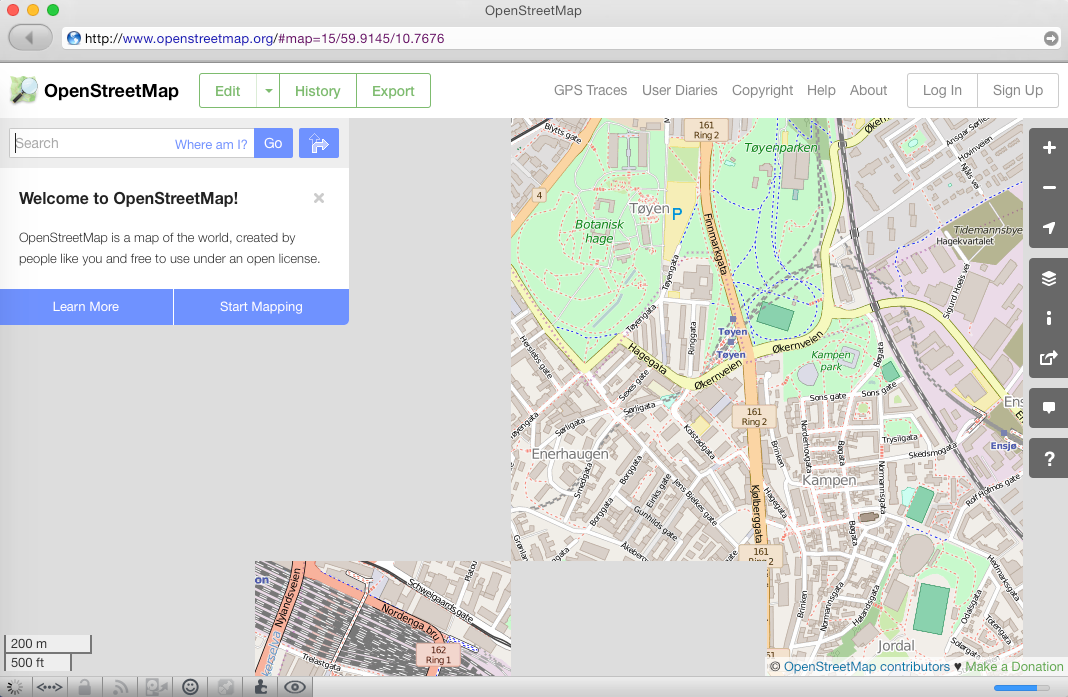
\includegraphics[width=\ScaleIfNeeded]{../chapter2/osm-org}
    \caption{Projekt-Homepage von OpenStreetMap während des Ladevorgangs}\label{fig:osm.org}
\end{figure}

Wegen der sehr großen Anzahl von Kacheln werden diese in größeren Maßstäben \term{just in time} gezeichnet. Die Kartenbasis ist für alle Maßstäbe die jeweils minutengenau aktualisierte OSM-Datenbank. \noref % evtl. Verweis auf RT09, insb. für basis, minutengenau -> p. 157 zu osmarender, -> p. 195 zu diffs
% just in time: http://wiki.openstreetmap.org/wiki/Mod_tile

Diese schnelle Aktualisierung ist für OpenStreetMap besonders wichtig, um den freiwillig Mitwirkenden nach einem Beitrag zur Datenbank ein schnelles Erfolgserlebnis zu geben, indem der Beitrag in der Karte weltweit für jeden sofort sichtbar wird.
Aus diesem Grund muss jede Generalisierung der Karte automatisiert ablaufen. Weiterhin bedeutet die Zahl der Beiträge mit teilweise über 1000 \term{changesets} pro Stunde, \cf{osm15}
% http://osmstats.neis-one.org/?item=changesets&date=7-11-2015
% http://neis-one.org/2013/08/osm-activity-report-2013/
dass der Arbeitsaufwand für eine manuelle Generalisierung prohibitiv hoch wäre. Klassische kartographische Generalisierung von Hand kommt daher nur für nicht nachzuführende und geographisch begrenzte Einzelanfertigungen in Betracht, etwa wenn auf Basis von OpenStreetMap eine traditionelle gedruckte Karte hergestellt werden soll.

Typischerweise besteht die Grundlage für Web-Karten wie derjenigen auf \url{osm.org} aus einer Geodatenbank, die mit einer Kopie der OpenStreetMap-Datenbank gefüllt und anschließend minütlich aktualisiert wird. Diese Geodatenbank enthält die Geometrie und Attribute der Rohdaten. Vom Kartenleser in der interaktiven Oberfläche im Webbrowser erzeugte Anfragen nach Kacheln der Karte werden dann von der Renderer-Software unter Zugriff auf die Geodatenbank abgearbeitet, wobei die Geometrie anhand der vorgegebenen Zeichenregeln dargestellt wird. Gerenderte Kacheln werden gecacht und zum Browser geschickt.

Eigene Bearbeitungsschritte zur Generalisierung von Daten sind bei diesem Ablauf nicht vorgesehen (im Gegensatz zu den Abläufen im AAA-Modell der deutschen Landesvermessung \cf[263, KN 62 (5)]{ML12}). Lediglich als Nebeneffekt des Einlesens in die Datenbank und des Zeichnens durch den Renderer wird eine begrenzte Modell-\noncf[194 17.2]{RT09} bzw. kartographische Generalisierung durchgeführt. \cf[194, 198]{RT09}
% [ML12] beschreibt einzelne kommerzielle Lösung (hat aber nette Bilder); -> möglichst noch bessere Quelle suchen
% http://wiki.openstreetmap.org/wiki/Mod_tile/Setup_of_your_own_tile_server

% Skizze OSM-Datenfluss

\begin{figure}[ht]
    \centering
    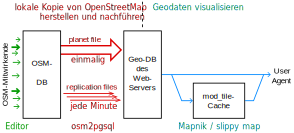
\includegraphics[width=\ScaleIfNeeded]{../chapter2/osm-datenfluss}
    \caption{OSM-Datenfluss}\label{fig:osm-datenfluss}
\end{figure}

% mapnik nur ein beispiel


% obiges trifft auf Linien, Punkte, Flächen gleichermaßen zu; hier darauf eingehen?


% LVAs verwenden (?) kartographische Hints, um die Ableitung von FOlge-DLMs zu erleichtern (?) [ML12, KN 62 (5) 263]. Das geht bei OSM nicht, weil auch das eben die Generalisierung und damti auch die Kartenherstellung verzögern und somit das schnelle ERfolgserlebnis verhindern würde. Es muss eben tatsächlich vollautomatisch ablaufen, wie auch immer.

% lesen: -> KN 56 (4) 191ff Modellgeneralisierung in ATKIS


%\begin{itemize}
%	\item erklären, wie die OSM-Rendering-Pipeline funktioniert, denn zum Verständnis von 2.3 ist wichtig, dass der Renderer die Geometrie nicht ändern kann
%\end{itemize}

% MapCSS includes an eval function, and has rules that act as 'commands' to modify data. CartoCSS does not support eval or any data-modifying operations.
% https://gist.github.com/tmcw/4319642


%\begin{itemize}
%	\item bisher im Wesentlichen nur automatische, (fast) ungeneralisierte Mercator-Tiles fürs Web
%	\item Datenmenge, Maßstäbe, ständige Änderungen und Aktualisierungen etc.
%	\begin{itemize}
%		\item manuelle Generalisierung ist nicht zielführend außer für nicht nachzuführende Einzelanfertigungen
%	\end{itemize}
%	\item in der Praxis fast nur einfache semantische Modellgeneralisierung unmittelbar im Tile-Renderer, keine kartographische Generalisierung oder Folgekarten bzw. -datenbanken
%	\begin{itemize}
%		\item nahe beieinander liegende Punktsignaturen werden willkürlich selektiert, Linearsignaturen überdecken einander
%	\end{itemize}
%	\item insbesondere kaum Vereinfachung, Qualitätsumschlag, Zusammenfassung oder Verdrängung (jedoch einige lohnenswerte Ansätze, z. B. \cf{MWG12} oder Haltestellen-Relationen {z. B. Konrad-Adenauer-Platz Beuel})
%\end{itemize}

% Angesichts dessen wären automatisiert abgeleitete, generalisierte Datenbanken für kleinere Maßstäbe zur Weiterverwendung wünschenswert, existieren jedoch bisher nicht. Entsprechend sind auch die aus OSM-Daten hergestellten Karten in aller Regel nicht kartographisch generalisiert: Nahe beieinander liegende Objekte überdecken einander scheinbar wahllos, Mindestgrößen und notwendige Formvereinfachungen werden von den automatischen Renderern ignoriert.

% Erschwert wird die Generalisierung von OSM-Daten unter anderem durch den hohen Grad der Fragmentierung von Linienzügen. Das Verknüpfen solcher zusammengehörenden, einzelnen ways durch Relationen in der Datenbank ist technisch möglich, wird aber von den Mitwirkenden aus unterschiedlichen Gründen nur sehr selten durchgeführt. Eine automatisierte Generalisierung durch Formvereinfachung (zur Reduktion der node-Anzahl) bedingt daher, dass die zusammengehörenden ways  dabei  als solche identifiziert werden. Gleiches gilt für die Generalisierung durch Zusammenfassung oder Verdrängung parallel verlaufender Linienzüge, beispielsweise Straßen mit begleitendem Radweg oder mehrgleisigen Bahnstrecken.



\section{Automatisierte Linien-Generalisierung von OpenStreetMap-Daten}

Wie im Folgenden einige Beispiele zeigen, lassen sich Auswahl auf Basis der Objektklasse sowie Betonung und Vergrößerung durch veränderte Strichbreite vergleichsweise einfach im Renderer implementieren, da die Geometrie der zugrundeliegenden Geodaten dabei unverändert bleibt. Andere Arten kartographischer Generalisierung wie etwa die Formvereinfachung oder der Qualitätsumschlag verändern die Geometrie und sind damit schwieriger zu implementieren.

\subsection{Generalisierung durch Objektauswahl}

Zur Herstellung der Kacheln der Web-Karte wird notwendigerweise für jede \term{Zoomstufe} eine Auswahl der jeweils  darzustellenden Objektklassen vorgenommen. Beispielsweise werden Anliegerstraßen \term{(residentials)} unterhalb von \term{zoom}~12 nicht mehr dargestellt (Abbildungen~\ref{fig:kampen11} und~\ref{fig:kampen12}). Dies vereinfacht das Kartenbild für den Betrachter und verringert die zu berechnende Datenmenge für den Renderer.

% Qualitätsumschlag fällt in OSM tlws. auch hierunter, gibt's aber nur für Flächen

% screenshots residentials z12 + z11

\begin{figure}[ht]
  \begin{minipage}{.5\linewidth}
    \centering
    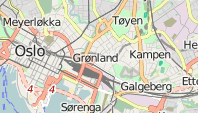
\includegraphics[width=\ScaleIfNeeded]{../chapter2/kampen-z12}
    \caption{Oslo, \term{zoom} 12}\label{fig:kampen12}
  \end{minipage}%
  \begin{minipage}{.5\linewidth}
    \centering
    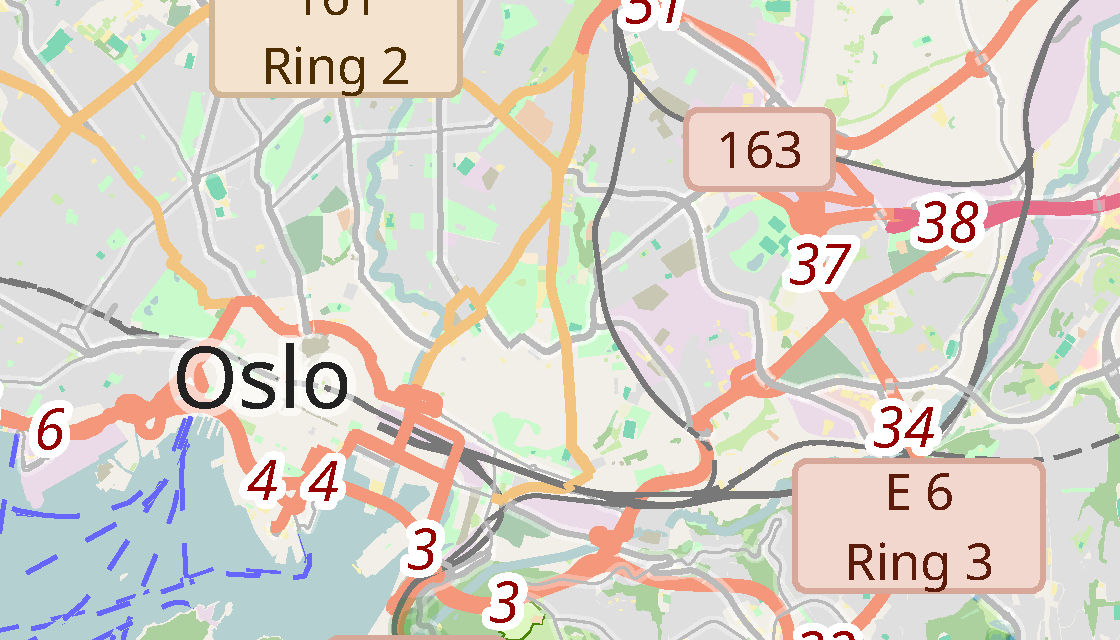
\includegraphics[width=\ScaleIfNeeded]{../chapter2/kampen-z11}
    \caption{Oslo, \term{zoom} 11}\label{fig:kampen11}
  \end{minipage}
\end{figure}




%\begin{figure}[ht]
%  \begin{minipage}{.5\linewidth}
%    \centering
%%    \rule{4cm}{3cm}
%    \includegraphics[width=\ScaleIfNeeded]{../chapter2/test}
%    \caption{Ein Rechteck akudbf sku fbskf bsd fdfb d f,df b dsz bf,ds f,sdzbg sb, fgs fgxh gxh gh}\label{fig:rechteck1}
%  \end{minipage}%
%  \begin{minipage}{.5\linewidth}
%    \centering
%    \captionaboveof{table}
%    [Maße des Rechtecks aus Abbildung~\ref{fig:rechteck1}]%
%    {Maße des Rechtecks}
%    \label{tab:rechteck1}
%    \begin{tabular}{ll}
%      Breite: & 4\,cm\\
%      Höhe: & 3\,cm
%    \end{tabular}
%  \end{minipage}
%\end{figure}

%\includegraphics[width=\ScaleIfNeeded]{../chapter2/test}




\subsection{Generalisierung durch Bewertung}


Weiterhin wird durch die Wahl der Zeichenregeln eine Bewertung der tatsächlich dargestellten Objekte vorgenommen, auch dies abhängig vom Maßstab. So werden Anliegerstraßen auf \term{zoom}~12 als schmaler, einfacher Strich gezeichnet, ab \term{zoom}~13 jedoch als weißer Breitstrich mit grauem Rand (Abbildungen~\ref{fig:kampen12} und~\ref{fig:kampen13}).

% Ist dies Bewertung? Sicherstellen in HGM02 o. ä.
% Hake, Grünreich, Meng 2002 Kartographie (8)

% screenshots residentials z14 + z13

\begin{figure}[ht]
  \begin{minipage}{.5\linewidth}
    \centering
    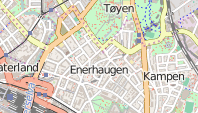
\includegraphics[width=\ScaleIfNeeded]{../chapter2/kampen-z13}
    \caption{Oslo, \term{zoom} 13}\label{fig:kampen13}
  \end{minipage}%
  \begin{minipage}{.5\linewidth}
    \centering
    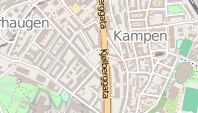
\includegraphics[width=\ScaleIfNeeded]{../chapter2/kampen-z14}
    \caption{Oslo, \term{zoom} 14}\label{fig:kampen14}
  \end{minipage}
\end{figure}


\subsection{Generalisierung durch Vergrößerung}

Die Wahl der Zeichenregeln beinhaltet für einige Objektklassen auch eine Generalisierung durch Vergrößerung, indem für bestimmte Maßstäbe eine Strichbreite gewählt wird, welche im Abbildungsmaßstab die tatsächliche Größe des Objekts übersteigt. Anliegerstraßen haben für die \term{Zoomstufen} 14 bis 19 jeweils eine unterschiedliche Strichbreite von $\unit[3]{px}$ bis $\unit[17]{px}$ definiert, so dass die Darstellung der Straße in der Karte Maßstabsänderungen andeutungsweise folgt (Abbildungen~\ref{fig:kampen17} und~\ref{fig:kampen14}). Die Breite von $\unit[3]{px}$ auf \term{zoom} 14 entspräche ca.~$\unit[27]{m}$ in der Realität \cf[155]{RT09}. Auf \term{zoom} 13 werden Anliegerstraßen gar auf dieselbe Breite von $\unit[3]{px}$ gezeichnet (ca.~$\unit[57]{m}$) und damit deutlich vergrößert, um die Erkennbarkeit im kleinerem Maßstab zu fördern (Abbildungen~\ref{fig:kampen14} und~\ref{fig:kampen13}).

% screenshots residentials z19 o. ä. + CartoCSS/MapCSS-mockup:
% https://github.com/gravitystorm/openstreetmap-carto/blob/fe4f8d48757cf85bb692129b5d9755ba5cadbbee/roads.mss
%@residential-width-z13:           3;
%@residential-width-z14:           3;
%@residential-width-z15:           5;
%@residential-width-z16:           6;
%@residential-width-z17:          12;
%@residential-width-z18:          14;
%@residential-width-z19:          21;

\begin{figure}[ht]
    \centering
    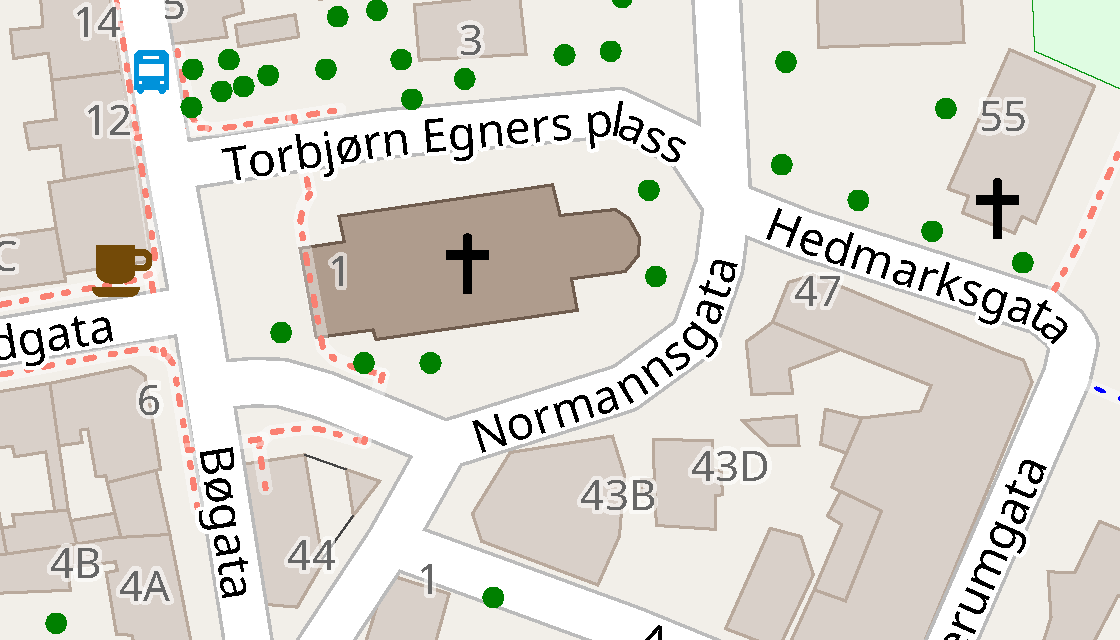
\includegraphics[width=\ScaleIfNeeded]{../chapter2/kampen-z17}
    \caption{Oslo, \term{zoom} 17}\label{fig:kampen17}
\end{figure}

\subsection{Generalisierung durch Formvereinfachung}

% grafik zur fragmentierung?
% grafik zum flussbett?

Eine kartographische Formvereinfachung wird für die Web-Karte nicht vorgenommen. Zufriedenstellende voll automatisiert arbeitende Algorithmen dafür stehen nicht zur Verfügung und ein Eingreifen von Hand ist wie zuvor in Abschnitt \ref{kartenherstellung} erläutert nicht vorgesehen.
% zB Trollstigen - Screenshots auch mit Vergleich zu Kartverket! http://arne.johannessen.de/osm/geocode-adapter/kartverket/?lat=62.459954&lon=7.6703534&zoom=15&layers=B
% zB Lahntalbahn http://www.openstreetmap.org/#map=7/51/8
% "kartographische Formvereinfachung" erklären?

Um die Kosten der Verarbeitung zu senken, ist für geometrische Daten oftmals eine Verringerung der Anzahl der Stützpunkte von Linien wünschenswert. Dies betrifft auch \osm. Entsprechende Algorithmen wie etwa Ramer-Douglas-Peucker [\noref DP73, zt. n. HS92] berücksichtigen jedoch oftmals nur die einzelne Linie unter Vernachlässigung der Netztopologie (Abbildungen~\ref{fig:kardemomme} und~\ref{fig:bab3}).

\begin{figure}[ht]
  \begin{minipage}{.5\linewidth}
    \centering
    \includegraphics[width=\ScaleIfNeeded]{../chapter2/kardemomme}
    \caption{Topologieverlust}\label{fig:kardemomme}
  \end{minipage}%
  \begin{minipage}{.5\linewidth}
    \centering
    \includegraphics[width=\ScaleIfNeeded]{../chapter2/bab3-a}
    \caption{Überkreuzen paralleler Linienzüge}\label{fig:bab3}
  \end{minipage}
\end{figure}

Ein weiteres Hindernis stellt die Fragmentierung der \osm-Linien dar. Bevor etwa über den Ramer-Douglas-Peucker eine nennenswerte Verringerung der \term{node}-Anzahl erreicht werden kann, müssen zunächst die einzelnen \term{ways} entlang des zu vereinfachenden Linienzugs miteinander verknüpft werden.

%Im Übrigen führt eine Verringerung der Zahl der Stützpunkte nicht notwendigerweise zu einer gelungenen kartographischen Generalisierung. Beispielsweise hatten Douglas und Peucker das Ziel \noref{Spekulation}, anhand eines mathematischen Verfahrens die Datenverarbeitung zu vereinfachen, während der sichtbare Linienverlauf nur so wenig wie möglich verändert werden sollte. Von einer Generalisierung nach dem kartographischen Gesichtspunkt „Signifikantes und Repräsentatives bewahren“ ist das Ergebnis regelmäßig weit entfernt. \noref

\begin{itemize}
%	\item Problem bei Formvereinfachung: Fragmentierung sowie Erhalten der geometrischen Topologie
	\item Beispiel: Fluss außerhalb des (unabhängig gemappten) Flussbetts \cf[57]{Kla11}
		\item ebenso bei als Flächen gemappten Straßen oder bei landuse=railway
	\item Beispiel: ungleichmäßiger Abstand (teils sogar negativ, d. h. Überkreuzen) paralleler Fahrbahnen oder Gleise (Skizze oder Screenshot)

	\item zumindest letzteres Beispiel ist lösbar durch vorhergehendes Zusammenfassen
	
	\item Aus diesen Gründen ist Formvereinfachung in kartographisch relevantem Ausmaß nur bei ganzheitlichem Ansatz sinnvoll, der alle Objektklassen berücksichtigt und sie zueinander passend generalisiert. Beispielsweise müsste der Verlauf einer in einem engen Flusstal verlaufenden Straße in gleicher Weise vereinfacht werden wie der Verlauf des Flusses. Wenn nötig, müsste eines dieser beiden Objekte dazu auch verdrängt werden. \cf[90][\? evtl.]{skg02} Ein derart aufwändiger Vorgang wird nicht von dem für die Web-Karte genutzten Renderer Mapnik implementiert. Es wäre ein separater vorgeschalteter Schritt notwendig, welcher aus der lokalen ungeneralisierten Geodatenbank eine separate generalisierte Geodatenbank erzeugt, die dann von Mapnik gerendert werden könnte. Dies ist derzeit nicht der Fall.
\end{itemize}


\subsection{Generalisierung durch Verdrängung}

Typisch für Web-Karten ist das völlige Fehlen von Verdrängungen zur Einhaltung kartographischer Minimalabstände und -dimensionen. Statt dessen werden mit kleiner werdendem Maßstab Objekte dichter und dichter aneinander, schließlich gar übereinander gezeichnet, worunter das Kartenbild teils erheblich leidet (Abbildung~\ref{fig:verdraengung}). Web-Karten mit \osm-Daten sind hier keine Ausnahme.

\begin{figure}[ht]
    \centering
    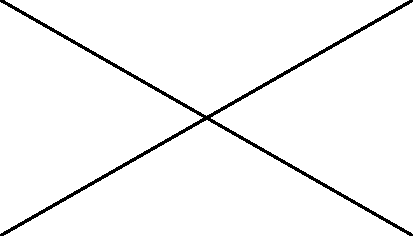
\includegraphics[width=\ScaleIfNeeded]{../image-missing}
    \caption{Typisches Generalisierungsergebnis in Web-Karten; fiktives Beispiel nach [sgk02, 49]}\label{fig:verdraengung}
\end{figure}

% Bevor eine Generalisierung durch Verdrängung stattfinden kann, muss zunächst der ohne Verdrängung entstehende Konflikt [das Hindernis] erkannt werden.
% Skizze zur Erläuterung (?)


\subsection{Generalisierung durch Zusammenfassung}

\begin{itemize}
%	\item hier: ohne Flächen zu berücksichtigen, obwohl dort evtl. ähnliche Probleme auftreten könnten
% (ich glaube, ähnliche Probleme treten eigentlich nicht auf)
	
%	\item Auswahl, Vergrößern und Betonen funktioniert zufriedenstellend
%		\item einfache Screenshots aus osm.org als Beispiele
	
	\item Problem bei Zusammenfassung: Linienzüge müssen (oft?) als zusammengehörig (z. B. parallel) erkannt werden, bevor zusammengefasst werden kann
	
	% Qualitätsumschlag? railway=rail -> landuse=railway ?
	
\end{itemize}


\section{Zielsetzung der Arbeit}

%\textbf{offener Punkt: Redundanz mit Themenblatt}

% Gedankensprung!
% (die Beispiele wiederholen sich => bessere Abgrenzung der Kapitel)

\begin{itemize}
	% „Algorithmen zur automatisierten Generalisierung durch Zusammenfassung von Linienzügen in OpenStreetMap“
	
	\item Erkennung als parallel ist bisher ein Problem
	
	\item Beispiel: Eisenbahnkarte mit untauglicher Darstellung von ein- und mehrgleisigen Strecken
		\item einfacher Screenshot von \\ \url{http://www.itoworld.com/map/231?lon=8.06752&lat=49.22313&zoom=9}
	
	\item ein Problem nicht nur in kleinen, sondern auch in großen Maßstäben:
	
	\item Beispiel: unregelmäßige Lücken zwischen Autobahn-Richtungsfahrbahnen
		\item einfacher Screenshot von osm.org
	
	\item Formvereinfachungen von Parallelen ist ungelöst
	% ||
	\item Beispiele: untaugliche Formvereinfachungen (kurzer Verweis auf vorgenannte Probleme)
	% nur hier nennen...? -> bessere Kapitelabgrenzung!
	
	\item \eyecatcher{Ziel der Arbeit:} die automatisierte Generalisierung durch Zusammenfassung von Linienzügen
	
	\item Visionen:
	\begin{itemize}
		\item kartographische Generalisierung => besseres Kartenbild
			\item Zusammenfassung der Attribute derart, dass die Möglichkeit zur Darstellung der Gesamtwerte besteht (z. B. Railway-Tracks / lanes)
		\item Verringerung der Datenmenge => einfacheres Arbeiten mit Daten für große Gebiete, Vereinfachung der Weiternutzung
			(möglichst Zahlenbeispiele für Dateigröße, Featurezahl und/oder Laufzeiten anhand meiner Skripte für größere OSM-Datensätze nennen)
		\item Zusammenfassung kann theoretisch auch das Erstellen von MRDBs vereinfachen
	\end{itemize}
	
	\item \emph{nicht} Teil der Arbeit sind insbesondere:
	\begin{itemize}
		\item die Formvereinfachung selbst
		\item eine wie auch immer geartete Verdrängung (obgleich eine solche durch diese Arbeit vielleicht erleichtert werden könnte)
	\end{itemize}
\end{itemize}


\section[Diskussion existierender Ansätze]{Diskussion existierender Ansätze zur automatisierten Linien-Generalisierung}

\begin{itemize}

	% ! Puffer
	\item Puffer \cf[2–3]{OHSZ10}
% - für eine Darstellung von OSM-Daten als Teil eiens 3D-Modells werden Straßen "realistisch" verbreitert per Buffer in PostGIS
% - um Fragmente und Parallelen zu beseitigen, werden die so entstandenen Polygone nun vereinigt
% => Parallelen finden durch Buffer-Algorithmus und Polygonanalyse
% => Epsilon benötigt
% - Buffer orthogonal zur Linie würde reichen; die Endrundungen können wegfallen
% - löst Zusammenfassung nicht; evtl. inward offset (um wieviel?) oder eher -> Skeleton

	% ! Skeleton
	\item Skeleton \cf{LM96} \cf{Mig12} \cf[][\?]{All11}

% Mig12: <http://mike.teczno.com/notes/osm-us-terrain-layer/foreground.html>
% <http://twak.blogspot.de/2009/01/that-straight-skeleton-again.html>
% <http://www.ikg.uni-hannover.de/skalen/buendel/PDF/Skeleton.pdf>

	% ! OS MasterMap
	\item OS MasterMap
	% \cf{CM05}
	\cf{Tho05}

	% ! Strokes
	\item Strokes \cf{Tho06b} \cf{EM00}

	% ! graphbasiert
	\item graphbasiert \cf{JC04} \cf{MM99} \cf{HAS05} \cf{TR95} \cf{Kne09}

	% ! Relational Constraints
	\item Relational Constraints \cf{TBDJRG12}

	% ! Conflict Detection
	\item Conflict Detection \cf{KP98} \cf{Tho06a}

	% ! -> Christian Stern
	\item …

\end{itemize}

% + RoadMatcher 
% <http://wiki.openstreetmap.org/wiki/Roadmatcher>
% + http://sourceforge.net/projects/jump-pilot/files/OpenJUMP_plugins/More%20Plugins/Matching%20PlugIn/
% <http://sourceforge.net/projects/jump-pilot/files/OpenJUMP_plugins/More%20Plugins/Matching%20PlugIn/>

(jeweils einschließlich Anwendbarkeit auf die vorliegende Fragestellung, ggf. Vor- und Nachteilen, ggf. Bezug der darin verwendeten Fachsprache zur in dieser Arbeit verwendeten Terminologie)



\nocite{*}  % include works in bibliography that aren't cited anywhere in the document (for debugging)

% single-chapter commands
\listoffigures %\listoftables
\bibliographystyle{../myAMSalpha} \bibliography{../thesis}{}
\end{document}
